%%%%%%%%%%%%%%%%%%%%%%%%%%%%%%%%%%%%%%%%%
% Journal Article
% LaTeX Template
% Version 1.3 (9/9/13)
%
% This template has been downloaded from:
% http://www.LaTeXTemplates.com
%
% Original author:
% Frits Wenneker (http://www.howtotex.com)
%
% License:
% CC BY-NC-SA 3.0 (http://creativecommons.org/licenses/by-nc-sa/3.0/)
%
%%%%%%%%%%%%%%%%%%%%%%%%%%%%%%%%%%%%%%%%%

%----------------------------------------------------------------------------------------
%	PACKAGES AND OTHER DOCUMENT CONFIGURATIONS
%----------------------------------------------------------------------------------------

\documentclass[12pt]{article}

\usepackage{lipsum} % Package to generate dummy text throughout this template
\usepackage[utf8x]{inputenc}
\usepackage[T1]{fontenc}
\PrerenderUnicode{áéíóúñ}
%\usepackage[spanish]{babel}
%\usepackage{t1enc}
\usepackage[english]{babel}
\usepackage{graphicx}
\usepackage{sidecap}
\usepackage{amssymb,amsmath}
\usepackage{mathtools}
\usepackage{amsmath}
\usepackage{mathrsfs}
\usepackage{float} 
\usepackage[sc]{mathpazo} % Use the Palatino font
\usepackage[T1]{fontenc} % Use 8-bit encoding that has 256 glyphs
\linespread{1.05} % Line spacing - Palatino needs more space between lines
\usepackage{microtype} % Slightly tweak font spacing for aesthetics
\usepackage{url}
\usepackage[hmarginratio=1:1,top=25mm,columnsep=25pt,left=20mm]{geometry} % Document margins
\usepackage{multicol} % Used for the two-column layout of the document
\usepackage[hang, small,labelfont=bf,up,textfont=it,up]{caption} % Custom captions under/above floats in tables or figures
\usepackage{booktabs} % Horizontal rules in tables
\usepackage{float} % Required for tables and figures in the multi-column environment - they need to be placed in specific locations with the [H] (e.g. \begin{table}[H])
\usepackage{hyperref} % For hyperlinks in the PDF
\usepackage{caption}
\usepackage{lettrine} % The lettrine is the first enlarged letter at the beginning of the text
\usepackage{paralist} % Used for the compactitem environment which makes bullet points with less space between them
\def\textsubscript#1{\ensuremath{_{\mbox{\textscale{.6}{#1}}}}}
\usepackage{abstract} % Allows abstract customization
\renewcommand{\abstractnamefont}{\normalfont\bfseries} % Set the "Abstract" text to bold
\renewcommand{\abstracttextfont}{\normalfont\small\itshape} % Set the abstract itself to small italic text
\usepackage{titlesec} % Allows customization of titles
\graphicspath{ {pics/} }
\titleformat{\section}[block]{\large\scshape\centering}{\thesection.}{1em}{} % Change the look of the section titles
\titleformat{\subsection}[block]{\large}{\thesubsection.}{1em}{} % Change the look of the section titles
\renewcommand{\labelitemi}{$\bullet$}
\renewcommand{\labelitemii}{$\cdot$}
\renewcommand{\labelitemiii}{$\diamond$}
\renewcommand{\labelitemiv}{$\ast$}


%\usepackage{fancyhdr} % Headers and footers
%\pagestyle{fancy} % All pages have headers and footers
%\fancyhead{} % Blank out the default header
%\fancyfoot{} % Blank out the default footer
%\fancyhead[C]{Metallicity Gradients in ies $\bullet$ December 2015} % Custom header text
%\fancyfoot[RO,LE]{\thepage} % Custom footer text

%----------------------------------------------------------------------------------------
%	TITLE SECTION
%----------------------------------------------------------------------------------------

\title{\vspace{-20mm}\fontsize{16pt}{10pt}\selectfont\textbf{Continuum determination}} % Article title

\author{
%\large
\textsc{Lynge R. B. Lauritsen} \\
\normalsize University of Copenhagen \\ % Your institution
\date{March 2018}
\vspace{-9mm}
}
%----------------------------------------------------------------------------------------

\usepackage{amsmath}
\begin{document}
%\begin{multicols}{1}
\maketitle % Insert title
%\end{multicols}{}

%\thispagestyle{fancy} % All pages have headers and footers

%----------------------------------------------------------------------------------------
%	ABSTRACT
%----------------------------------------------------------------------------------------

%\begin{abstract}

%\noindent ABSTRACT

%\end{abstract}

%----------------------------------------------------------------------------------------
%	ARTICLE CONTENTS
%----------------------------------------------------------------------------------------
%\begin{multicols}{2} % Two-column layout throughout the main article text

\section{Finding Continuum}
In this section the process utilised in determining the used continuum destribution of the observed quasar data is described. The method used was found through a combination of reading relevant literature and implementation of numerical MCMC algorithm. At no point in this endeavor has the aim been to find the absolute Continuum Light Curve (CLC). The objectively correct CLC is of no real importance in the investigation, and therefore would cause unnecessary time to pursue. The difficulty in determining the absolute CLC is in the lack of knowledge of the actual band dependent transfer function of the observed Light Curves (LC). Additionally the interest in the project is the timelag between the observable bands, and as such the relative transfer functions as opposed the the absolute transfer functions. \\
This section will be focused upon describing the methods used and the reasons behind the decisions taken.\\

\section{Defining a Light Curve}
Three main methods of characterising Light Curves has been explored during the course of this project. Each methods have their own advantages and disadvantages, and to accurately formulate a working model for the continuum Light Curve all three has been utilised. The methods are;
\begin{enumerate}
\item The Stochastic model described in Kelly et al. (2009). This model builds on the assumption of AGN variability being described as a \emph{Continuous Time First-Order Autoregressive Process} (\emph{CAR(1)}).
\item Modeling the AGN variability as a Power Spectrum with Power Spectral Density slope of $\alpha=-2.3...-3.4$.
\item Using Structure Functions to analyse AGN variability.
\end{enumerate}
These three approaches allows for the identification and evolution of different aspects of AGN light curves. The Structure Function allows for the understanding of certain key characteristics of the observed and modeled Light-Curves, whereas both the Kelly et al. (2009) and the Power Spectrum approach allows for the modeling and evolution of AGN 

\subsection{Original Data Material and Kelly manipulations}
Light Curve sampling is dependent on atmospheric conditions, the visible night sky and observation time on the telescope. As such observed light-curves will often be unevenly sampled with time intervals of days or perhaps weeks. As such a method of modeling the missing data can be necessary, it is with this aim that the Kelly et al. (2009) described Stochastic model (from here named \emph{"Kelly model"}) is investigated. In the data obtained for the purpose of this project considerable and uneven time intervals presents itself. The Kelly model is a model build over the assumption that a Light-Curve observed in an AGN can be modeled as a \emph{Continuous Time First-Order Autoregressive} (\emph{CAR(1)}) \emph{Process}. The Kelly model is consistent with a power spectra of the form $P(f)=1/f^{2}$, this as described later, despite being a common assumption for AGN variability, is not an entirely accurate representation of the observed AGN variability, thus the Kelly model cannot, standalone, define an actual AGN Light-Curve without additional development. \\
\\
The Kelly model is, as mentioned, a Continuous Stochastic model, rather than modeling Liht-Curves using Fourier (Spectral) techniques. It is modeled as Continuous time as the physical processes occurring in the accretion disk is continuous and it provides a natural way of handling irregular sampling. The model uses 3 different parameters to define the Light-Curve created;
\begin{enumerate}
\item A characteristic time-scale, called the \emph{"relaxation time"} ($\tau_{Kelly}$)
\item Amplitude of short time-scale variability
\item Mean value of the Light-Curve
\end{enumerate}
The \emph{"relaxation time"} is given as the time-scale at which the time series becomes uncorrelated and is easily associated with the various characteristic time-scales inherent in the accretion disk physics such as the light crossing time, the orbital time-scale and the thermal time-scale.
\begin{equation}
t_{lc} = 1.1\times(\frac{M_{BH}}{10^{8}M_{O}})(\frac{R}{100R_{S}})~days
\label{eq:t_lc}
\end{equation} 
\begin{equation}
t_{lc} = 104\times(\frac{M_{BH}}{10^{8}M_{O}})(\frac{R}{100R_{S}})^{3/2}~days
\label{eq:t_orb}
\end{equation} 
\begin{equation}
t_{lc} = 4.6\times(\frac{\alpha}{0.01})^{-1}(\frac{M_{BH}}{10^{8}M_{O}})(\frac{R}{100R_{S}})^{3/2}~yr
\label{eq:t_th}
\end{equation} 
In Kelly et al. 2009 the relationship between the Characteristic time-scales in \emph{equations \ref{eq:t_lc}, \ref{eq:t_orb} and \ref{eq:t_th}} and the \emph{relaxation time} is investigated. They conclude that although both the $t_{orb}$ and the $t_{th}$ provides reasonable fits, the best fit is the thermal time-scale. The differential equation governing the $Kelly \ model$ is given through $equation$ \ref{eq:Kelly2009}.   

%The Kelly model builds on previous works identifying the Power Spectral Density Slope to be $\alpha \sim -2$, and inaccurate assumption as later described, 


%The CLC is found based upon the observed light curves of the K-band. The REM data is observed in the KHJgriz bands. The REM data is uneven in the sampling and subject to several observation gaps of a 50 - 100 day period. Due to this sampling it has proved of interest to attempt to simulate the Observed Light Curves (OLC) across the observational gaps. These has been filled through the use of the Kelly Function (Kelly et al. 2009). The Kelly Function is not actually a function as much as a way of approximating the next point of the LC based upon the overall distribution of observed values. It is given by \emph{equation \ref{eq:Kelly2009}},

\begin{equation}
dX(t) = -\frac{1}{\tau_{Kelly}}X(t)dt + \sigma\sqrt{dt}\epsilon(t) + bdt
\label{eq:Kelly2009}
\end{equation}
with $b\tau_{Kelly}$ being the observed mean value of the OLC and $\tau_{Kelly}$ is the relaxation time additionally the variance on the Light-Curve is given by $\tau\sigma^{2}/2$. Additionally the $\epsilon(t)$ a white noise function of zero mean and variance of one, and $X(t)$ represents the Light-Curve. The Kelly approach introduces a slight shifting on the axis dependent on the direction of evolution and the direction in which the Light-Curve is read. Due to this bias in the $Kelly \ model$ it has been chosen during the course of this project to generate the \emph{Kelly Light-Curve} from both directions and use the mean Light-curve. This is examplified in \emph{figure \ref{fig:NGC3783K-Kelly}}

\begin{figure}[t!]
\centering
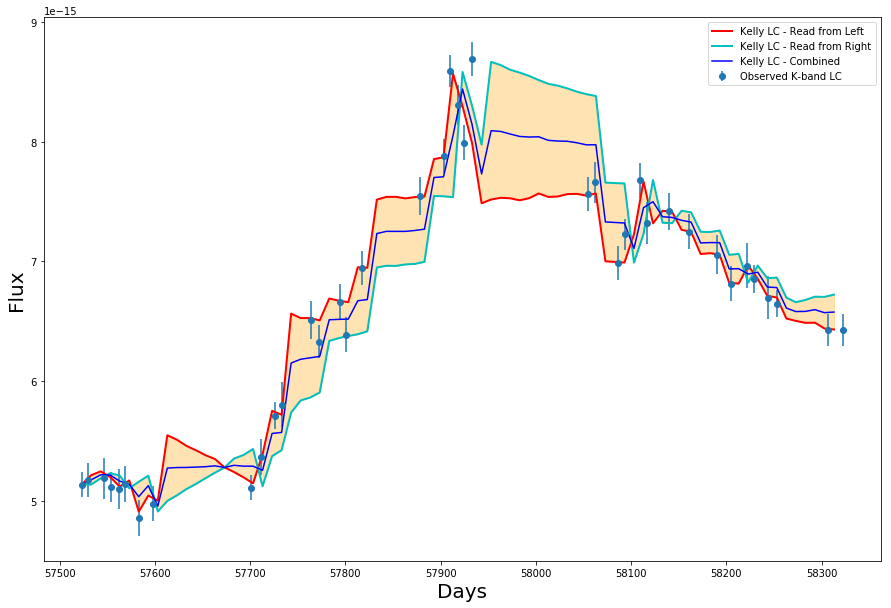
\includegraphics[width=1\linewidth]{Figure/NGC3783K-Kelly.png}\\
\caption{The Kelly function applied to the NGC3783 K-band spectrum. The red curve is the $Kelly \ method$ interpretation as applied from left to right, and the green is the opposing direction. It becomes apparent that significant bias can be found in the Kelly method as only applied in one direction.}
\label{fig:NGC3783K-Kelly}
\end{figure}

\noindent The three parameters defining the $Kelly \ model$ can be determined through the use of a maximum likelihood estimate from \emph{equations \ref{eq:p(b,sigma,tau)} through \ref{eq:a_i}}.
\begin{equation}
p(x_{1},...,x_{n}|b,\sigma,\tau) = \prod_{\mathclap{i=1}}^{\mathclap{n}}[2\pi(\Omega_{i}+\sigma_{i}^{2})]^{-1/2}\times exp[-\frac{1}{2}\frac{(\hat{x}_{i}-x_{i}^{*})^{2}}{\Omega_{i}+\sigma^{2}}]
\label{eq:p(b,sigma,tau)}
\end{equation}
\begin{equation}
x_{i}^{*} = x_{i}-b\tau_{Kelly}
\label{eq:x_star}
\end{equation} 
\begin{equation}
\hat{x}_{1} = 0
\label{eq:x_hat_1}
\end{equation} 
\begin{equation}
\Omega_{1} = \frac{\tau_{Kelly}\sigma^{2}}{2}
\label{eq:Omega_1}
\end{equation}
\begin{equation}
\hat{x}_{i>1} = a_{i}\hat{x}_{i-1}+\frac{a_{i}\Omega_{i-1}}{\Omega_{i-1}+\sigma_{i-1}^{2}}(x_{i-1}^{*}-\hat{x}_{i-1})
\label{eq:x_hat_i}
\end{equation}
\begin{equation}
\Omega_{i>1} = \Omega_{1}(1-a_{i}^{2})+a_{i}^{2}\Omega_{i-1}(1-\frac{\Omega_{i-1}}{\Omega_{i-1}+\sigma_{i-1}^{2}})
\label{eq:Omega_i}
\end{equation}
\begin{equation}
a_{i>1} = exp[-\frac{t_{i}-t_{i-1}}{\tau_{Kelly}}]
\label{eq:a_i}
\end{equation}
The $Kelly \ method$ as a $CAR(1)$ process has a power spectrum given by $equation \ ref{eq:Kelly_power_spectrum}$
\begin{equation}
P(f) = \frac{2\sigma^{2}\tau_{Kelly}^{2}}{1+(2\pi\tau_{Kelly}f)^{2}}
\label{eq:Kelly_power_spectrum}
\end{equation}
allowing the resulting Light-Curve to be separated in two different regimes. In the case of time-scales being short as compared to the $relaxation \ time$ the power spectrum falls as $1/f^{2}$ and in the case of time-scales longer than the $relaxation \ time$ the power spectrum becomes constant.  \\
\\
Analysing $figure$ \ref{fig:Kelly2009} one can identify one of the key weaknesses in the $Kelly \ method$ in the significant time-gaps displayed. The Kelly Function provides a generally reasonable fit in areas of reasonable coverage for the observations, however it proves unable to successfully predict reasonable suggested data for time-gaps of significant size. As such utilising the range of suggestions provided by the twin interpretations from opposing sides becomes useful. It may be possible to adjust this somewhat by introducing a dependence of time from the points of observation that the estimate is based upon. This however is not the focus at this time. 

\subsection{Power Spectral Density}'
The Power Spectral Density (PSD) is an expression of variability in a function as a function of temporal frequency. The PSD is determined by calculating a periodogram (\emph{equations \ref{eq:zero_freq}, \ref{eq:mod_squared_Fourier} and \ref{eq:Power_Spectra}}). The $periodogram$ resultant of calculating the Power Spectral Density of real observable data is an $inconsistent$ estimator of the PSD, as the scatter observed in the periodogram is not decreasing as the number of observations is increased, necessitating averaging the periodogram. This can be done by either binning the calculated frequencies, or averaging over data segments, thus allowing an averaged periodogram to become a $consistent$ estimator of the PSD (Vaughan et al. 2003) \\
\\
In the case of AGN Light-Curves the interesting aspect of the PSDs becomes the slope of the $consistent$ estimator. This PSD slope (denoted $\alpha$) can be an indication of the time-dependent variability of AGN Light-Curves should a general tendency be identified. It is important to acknowledge that AGNs vary and as such, despite early assumptions of $\alpha=2$ the PSD slope is not identical across observed AGNs.\\
\\
The PSD can be obtained from both evenly and unevenly sampled light-curves. To calculate the PSD from a discrete Light-Curve ($X(t_{i})$) with N observed data points it is necessary to remove the zero-frequency power, by subtracting the mean from the Light-Curve,
\begin{equation}
X_{PSD}(t_{i}) = X(t_{i}) - \mu(X(t_{i}))
\label{eq:zero_freq}
\end{equation} 
and calculate the modulus squared of the discrete Fourier transform
\begin{equation}
|F_{N}(\nu)|^{2} = [\sum_{{i=1}}^{N}X_{PSD}(t_{i})cos(2\pi\nu t_{i})]^{2} + [\sum_{{i=1}}^{N}X_{PSD}(t_{i})sin(2\pi\nu t_{i})]^{2}
\label{eq:mod_squared_Fourier}
\end{equation} 
with $\nu$ being the sampled frequencies of the discrete Fourier transform occuring at evenly spaced intervals at $\nu_{min}$, $2\nu_{min}$, $3\nu_{min}$,...,$\nu_{Nyq}$, with $\nu_{min} = T^{-1}$ (T being total length of Light-Curve) and $\nu_{Nyq}$ being the Nyquist frequency of $(2T/N)^{-1}$. The power of the relevant function is obtained by nomalising $|F_{N}(\nu)|^{2}$ (Uttley et al. 2001)
\begin{equation}
P(\nu) = \frac{2T}{\mu^{2}N^{2}}|F_{N}(\nu)|^{2}.
\label{eq:Power_Spectra}
\end{equation} 
This Power Spectra allows the integration of the Power Spectra over a range $\nu_{1}$ to $\nu_{2}$ to determine the contribution to the fractional rms squared variability ($\sigma^{2}/\mu^{2}$) of the Light-Curve generated by variations on the time-scale $T_{2}$ to $T_{1}$. (FIND AND CHECK van der Klis 1997). The total fractional rms variability observed is thus determined by the square root of the integrated power spectrum. It is observed in Uttley et al. 2001 that the actually observed power spectra for AGN demonstrate either a Knee Model power spectra, by flattening to a slope of $\alpha=0$ at low frequencies or a high-frequency break model (by flattening to a slope of $\alpha=1$ at low frequencies). \\
The PSD slope is obtained through linear fitting in loglog-space past the "Knee" or "Break". \\
\\
In a study by Smith et al. 2018 of 21 Type I AGN Light-Curves from Kepler the PSD slopes has been studied. The AGNs studied by Smith et al. 2018 are comparable to AGNs studied in this project, in them being of the local universe, all but one of them with redshift $z<1$. In the study it is determined that the PSD slope ($\alpha$) ranges from -1.7 to -3.4 with a mean value of $\alpha_{mean}=-2.51$ and standard deviation of $\alpha_{std}=0.42$. This allows for better indications of the Physical relevance of the generated driving function of the observed AGNs, that is attempted in this project. 
\subsection{Structure Function}
The structure function is used to understand the behavior of long-term AN variability. Short-term AGN variability is generally accepted to be attributed towards relativistic beaming effects (READ UP ON THIS AND WRITE EXPLANATION FOR THIS IN THEORY), however long-term AGN variability is more difficult to ascertain the cause of. Suggestions towards possible causes is (as given in Vries et al. 2004 and Kawaguchi et al. 1998):
\begin{enumerate}
\item Disk Instability (described in Starling et al. 2004 READ UP ON IT AND WRITE HERE)
\item Super Novae event bursts close to the AGN 
\item Source extrinsic variations due to microlensing events along line-of-sight
\end{enumerate}
The structure function, as described by Kawaguchi et al. (1998) and Simonetti et al. (1985) (FIND THIS PAPER), is given by $equation$ \ref{eq:structure_function}
\begin{equation}
V(\tau) = \frac{1}{N(\tau)}\sum_{\mathclap{i<j}}[m_{opt}(t_{i})-m_{opt}(t_{j})]^{2}
\label{eq:structure_function}
\end{equation}
with $m_{opt}(t_{i})$ being the optical magnitude at the time $t_{i}$, $\tau$ being the time-difference $t_{i}-t_{j}$ and $N(\tau)$ being number of pairs of $\tau = t_{i}-t_{j}$. The structure function itself applied to an observed AGN Light-Curve will demonstrate three regimes (Kawaguchi et al. 1998, Hughes et al. 1992 (FIND THIS PAPER AND CONFIRM));
\begin{enumerate}
\item A plateau at time-lags exceeding the longest correlation time-scale, with a value twice the variance of fluctuations in the measurements 
\item Plateau at short time-lags with value twice the measurement noise (not in models without arbitrary measurement noise)
\item Power-law increase with time-lag as $[V(\tau)]^{1/2}\propto \tau^{\beta}$ between the two plateau'
\end{enumerate}
Additionally there is a comparability between the PSD slope ($\alpha$), discussed previously, and the structure function slope ($\beta$) of $\alpha=1+2\beta$ assuming $1\le\alpha\le3$ (FIND REFERENCE EITHER KAWAGUCHI OR VRIES).

\subsection{Transfer Functions}
In order to determine the CLC one must have an understanding of how the LC behaves from the Quasar to the observation. If one were to determine the exact Transfer Function at all times, it would then be possible to determine the exact CLC. However the transfer function is an unknown quantity and as the OLC is the result of the transfer function and the OLC (\emph{equation \ref{eq:OLC}}) (Andreas Skielboe 2016)
\begin{equation}
F_l(t,\lambda) = \int_{-\infty}^{\infty}\Psi(\tau,\lambda)F_C(t-\tau)d\tau
\label{eq:OLC}
\end{equation}
it is impossible to accurately determine the CLC. However this project is not concerned with the accurate CLC, it is however interested in the relative difference between the Transfer Functions. It is therefore decided to assume a Transfer Function for the K-band data. Using this arbitrary function, \emph{equation \ref{eq:OLC}} and an MCMC algorithm a possible CLC is determined. This possible CLC can then be utilised in compound with the OLC for the renmaining observed bands and \emph{equation \ref{eq:OLC}} to determine the relative differences and hence the timelag between the Transfer Functions. \\
For arbitrary Transfer Function a log-normal is chosen (\emph{equation \ref{eq:TF}})
\begin{equation}
f(x) = \frac{1}{x\sigma\sqrt{2\pi}}e^{-\frac{(ln(x)-\mu)^2}{2\sigma^2}}
\label{eq:TF}
\end{equation}
The transfer function of an AGN however is not a simple singular log-normal function. In order to accurately determine the transfer function it is important to take into account the separate the individual transfer function contributions from the BLR and the Dusty Torus. The exact shape of the complete transfer function must thusly be a combination of the BLR and the Dust Torus contributions. The complete transfer function thus becomes
\begin{equation}
f(x) = A_{T}\frac{1}{x\sigma_{Dust}\sqrt{2\pi}}e^{-\frac{(ln(x)-\mu_{Dust})^2}{2\sigma_{Dust}^2}} - (1 - A_{T})\frac{1}{x\sigma_{BLR}\sqrt{2\pi}}e^{-\frac{(ln(x)-\mu_{BLR})^2}{2\sigma_{BLR}^2}},
\label{eq:TF}
\end{equation}
with $A_{T}$ being the fraction of the complete transfer function contribution originating from the dust torus. 

\subsubsection{BLR Transfer Function contribution}


\subsection{MCMC algorithm and reasoning}
The CLC is determined through an MCMC type algorithm. An initial guess for the CLC is made and the quality of the fit is made through the use of a variety of factors. 
\begin{enumerate}
\item Determining the residuals squared of the $F_l(t,\lambda)$
\item Determining the double derivative of the CLC
\item Determining the PSD slope of the CLC
\item Producing a Kelly fitting for the CLC
\end{enumerate}
The code then randomly alters the first point on the CLC and item 1 through 4 is redetermined and compared. In the case of a favorable outcome the alteration is saved and the code moves onwards to the following point. The favorability of an outcome is evalueated by a series of parameters. 
\begin{enumerate}
\item Residuals: In all cases the sum of the residuals squared must be less than the previous alteration.
\item Double Derivative: The double derivative is compared to the maximum rate of change of the OLC and is accepted if it is no more than 40 percent larger than the originally observed. This is done to prevent rapid changes to the CLC that would ultimately make for a more stable, but ultimately unphysical solution to the CLC. 40 percent has been chosen as it is felt that despite the OLC becoming somewhat more smooth as a result of the Transfer Function, it would be unlikely to be that prominent. The alternative is the sum of the change in the rate of change of beth adjacent points as well as the altered points decreases overall. This would be accepted as well, pending other factors.
\item PSD slopes: Assuming 1 and 2 holds true, the change can be accepted if the PSD slope is moving closer to the accepted slope, or inside 0.05 of the accepted (so as to allow some freedom of movement of the CLC).
\item Kelly: In the case of 1 holding true, and 2 follows the path of the set of double derivatives overall decreasing there will be a statistical possibility of 5 percent of a change being accepted IF the Kelly function provides an overall better fit and the PSD slope is no more than 0.3 out. This is done primarily to utilise the Kelly function as a method of approximating LC's and hence allowing for the use of this additional resource in providing a more physical fitting, as well as counterbalancing the possibility of the CLC becoming stable in an unstable equilibrium position due to the other limitations.
\end{enumerate}
It is being experimented upon with both one moving point as well as three. 
%----------------------------------------------------------------------------------------
%	REFERENCE LIST
%----------------------------------------------------------------------------------------
\newpage
[1] Kelly et al. 2009, APJ698:895-910 
[2] Kelly et al. 2009, arXiv:0903.5315v1 
[3] A. Skielboe 2016, Thesis 
[4] Uttley et al. 2002 Mon. Not. R. Astron. Soc. 332,231-250

%\end{multicols}
\end{document}
